\documentclass[11pt]{report}

\usepackage{indentfirst}
\usepackage[body={6in,8.5in}]{geometry}
\usepackage{hyperref}
\usepackage{graphicx}
\DeclareGraphicsRule{.ps}{eps}{}{}

\renewcommand{\thesection}{\arabic{section}}
\setcounter{tocdepth}{3}
\setcounter{secnumdepth}{3}

\begin{document}
\begin{center}
  {\Large LAPACK Working Note 81\\
  Quick Installation Guide for LAPACK on Unix Systems\footnote{This work was
 supported by NSF Grant No. ASC-8715728  and NSF Grant No. 0444486}}
\end{center}
\begin{center}
%  Edward Anderson\footnote{Current address:  Cray Research Inc.,
%                           655F Lone Oak Drive, Eagan, MN  55121},
  The LAPACK Authors\\
  Department of Computer Science \\
  University of Tennessee \\
  Knoxville, Tennessee  37996-1301 \\
\end{center}
\begin{center}
  REVISED:  VERSION 3.1.1, February 2007 \\
  REVISED:  VERSION 3.2.0, November 2008
\end{center}

\begin{center}
Abstract
\end{center}
This working note describes how to install, and test version 3.2.0
of LAPACK, a linear algebra package for high-performance
computers, on a Unix System.  The timing routines are not actually included in
release 3.2.0, and that part of the LAWN refers to release 3.0.  Also,
version 3.2.0 contains many prototype routines needing user feedback.
Non-Unix installation instructions and
further details of the testing and timing suites are only contained in
LAPACK Working Note 41, and not in this abbreviated version.
%Separate instructions are provided for the Unix and non-Unix
%versions of the test package.
%Further details are also given on the design of the test and timing
%programs.
\newpage

\tableofcontents

\newpage
% Introduction to Implementation Guide

\section{Introduction}

LAPACK is a linear algebra library for high-performance
computers.
The library includes Fortran subroutines for
the analysis and solution of systems of simultaneous linear algebraic
equations, linear least-squares problems, and matrix eigenvalue
problems.
Our approach to achieving high efficiency is based on the use of
a standard set of Basic Linear Algebra Subprograms (the BLAS),
which can be optimized for each computing environment.
By confining most of the computational work to the BLAS,
the subroutines should be
transportable and efficient across a wide range of computers.

This working note describes how to install, test, and time this
release of LAPACK on a Unix System.

The instructions for installing, testing, and timing
\footnote{timing are only provided in LAPACK 3.0 and before}
are designed for a person whose
responsibility is the maintenance of a mathematical software library.
We assume the installer has experience in compiling and running
Fortran programs and in creating object libraries.
The installation process involves untarring the file, creating a set of
libraries, and compiling and running the test and timing programs
\footnotemark[\value{footnote}].

%This guide combines the instructions for the Unix and non-Unix
%versions of the LAPACK test package (the non-Unix version is in Appendix
%~\ref{appendixe}).
%At this time, the non-Unix version of LAPACK can only be obtained
%after first untarring the Unix tar tape and then following the instructions in
%Appendix ~\ref{appendixe}.

Section~\ref{fileformat} describes how the files are organized in the
file, and
Section~\ref{overview} gives a general overview of the parts of the test package.
Step-by-step instructions appear in Section~\ref{installation}.
%for the Unix version and in the appendix for the non-Unix version.

For users desiring additional information, please refer to LAPACK
Working Note 41.
% Sections~\ref{moretesting}
%and ~\ref{moretiming} give
%details of the test and timing programs and their input files.
%Appendices ~\ref{appendixa} and ~\ref{appendixb} briefly describe
%the LAPACK routines and auxiliary routines provided
%in this release.
%Appendix ~\ref{appendixc} lists the operation counts we have computed
%for the BLAS and for some of the LAPACK routines.
Appendix ~\ref{appendixd}, entitled ``Caveats'', is a compendium of the known
problems from our own experiences, with suggestions on how to
overcome them.

\textbf{It is strongly advised that the user read Appendix
A before proceeding with the installation process.}
%Appendix E contains the execution times of the different test
%and timing runs on two sample machines.
%Appendix ~\ref{appendixe} contains the instructions to install LAPACK on a non-Unix
%system.

\section{Revisions Since the First Public Release}

Since its first public release in February, 1992, LAPACK has had
several updates, which have encompassed the introduction of new routines
as well as extending the functionality of existing routines.  The first
update,
June 30, 1992, was version 1.0a; the second update, October 31, 1992,
was version 1.0b; the third update, March 31, 1993, was version 1.1;
version 2.0 on September 30, 1994, coincided with the release of the
Second Edition of the LAPACK Users' Guide;
version 3.0 on June 30, 1999 coincided with the release of the Third Edition of
the LAPACK Users' Guide;
version 3.1 was released on November, 2006;
version 3.1.1 was released on November, 2007;
and version 3.2.0 was released on November, 2008.

All LAPACK routines reflect the current version number with the date
on the routine indicating when it was last modified.
For more information on revisions in the latest release, please refer
to the \texttt{revisions.info} file in the lapack directory on netlib.
\begin{quote}
\url{http://www.netlib.org/lapack/revisions.info}
\end{quote}

%The distribution \texttt{tar} file \texttt{lapack.tar.z} that is
%available on netlib is always the most up-to-date.
%
%On-line manpages (troff files) for LAPACK driver and computational
%routines, as well as most of the BLAS routines, are available via
%the \texttt{lapack} index on netlib.

\section{File Format}\label{fileformat}

The software for LAPACK is distributed in the form of a
gzipped tar file (via anonymous ftp or the World Wide Web),
which contains the Fortran source for LAPACK,
the Basic Linear Algebra Subprograms
(the Level 1, 2, and 3 BLAS) needed by LAPACK, the testing programs,
and the timing programs\footnotemark[\value{footnote}].
Users who wish to have a non-Unix installation should refer to LAPACK
Working Note 41,
although the overview in section~\ref{overview} applies to both the Unix and non-Unix
versions.
%Users who wish to have a non-Unix installation should go to Appendix ~\ref{appendixe},
%although the overview in section ~\ref{overview} applies to both the Unix and non-Unix
%versions.

The package may be accessed via the World Wide Web through
the URL address:
\begin{quote}
\url{http://www.netlib.org/lapack/lapack.tgz}
\end{quote}

Or, you can retrieve the file via anonymous ftp at netlib:

\begin{verbatim}
     ftp ftp.netlib.org
     login:  anonymous
     password:  <your email address>
     cd lapack
     binary
     get lapack.tgz
     quit
\end{verbatim}

The software in the \texttt{tar} file
is organized in a number of essential directories as shown
in Figure 1.  Please note that this figure does not reflect everything
that is contained in the \texttt{LAPACK} directory.  Input and instructional
files are also located at various levels.
\begin{figure}
\vspace{11pt}
\centerline{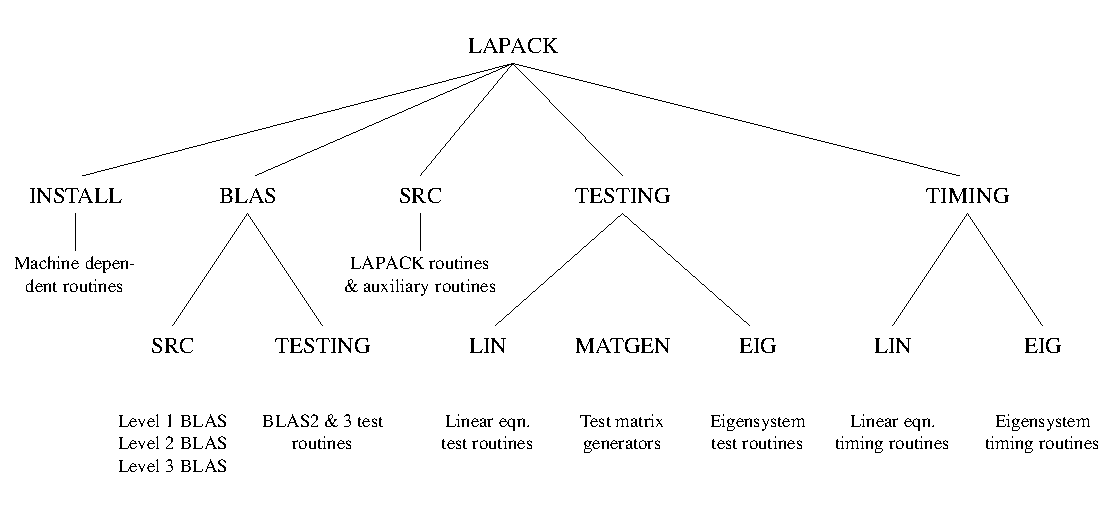
\includegraphics[width=6.5in,height=3in]{org2.ps}}
\caption{Unix organization of LAPACK 3.0}
\vspace{11pt}
\end{figure}
Libraries are created in the LAPACK directory and
executable files are created in one of the directories BLAS, TESTING,
or TIMING\footnotemark[\value{footnote}].  Input files for the test and
timing\footnotemark[\value{footnote}]  programs are also
found in these three directories so that testing may be carried out
in the directories LAPACK/BLAS, LAPACK/TESTING, and LAPACK/TIMING \footnotemark[\value{footnote}].
A top-level makefile in the LAPACK directory is provided to perform the
entire installation procedure.

\section{Overview of Tape Contents}\label{overview}

Most routines in LAPACK occur in four versions: REAL,
DOUBLE PRECISION, COMPLEX, and COMPLEX*16.
The first three versions (REAL, DOUBLE PRECISION, and COMPLEX)
are written in standard Fortran and are completely portable;
the COMPLEX*16 version is provided for
those compilers which allow this data type.
Some routines use features of Fortran 90.
For convenience, we often refer to routines by their single precision
names; the leading `S' can be replaced by a `D' for double precision,
a `C' for complex, or a `Z' for complex*16.
For LAPACK use and testing you must decide which version(s)
of the package you intend to install at your site (for example,
REAL and COMPLEX on a Cray computer or DOUBLE PRECISION and
COMPLEX*16 on an IBM computer).

\subsection{LAPACK Routines}

There are three classes of LAPACK routines:
\begin{itemize}

\item \textbf{driver} routines solve a complete problem, such as solving
a system of linear equations or computing the eigenvalues of a real
symmetric matrix.  Users are encouraged to use a driver routine if there
is one that meets their requirements.  The driver routines are listed
in LAPACK Working Note 41~\cite{WN41} and the LAPACK Users' Guide~\cite{LUG}.
%in Appendix ~\ref{appendixa}.

\item \textbf{computational} routines, also called simply LAPACK routines,
perform a distinct computational task, such as computing
the $LU$ decomposition of an $m$-by-$n$ matrix or finding the
eigenvalues and eigenvectors of a symmetric tridiagonal matrix using
the $QR$ algorithm.
The LAPACK routines are listed in LAPACK Working Note 41~\cite{WN41}
and the LAPACK Users' Guide~\cite{LUG}.
%The LAPACK routines are listed in Appendix ~\ref{appendixa}; see also LAPACK
%Working Note \#5 \cite{WN5}.

\item \textbf{auxiliary} routines are all the other subroutines called
by the driver routines and computational routines.
%Among them are subroutines to perform subtasks of block algorithms,
%in particular, the unblocked versions of the block algorithms;
%extensions to the BLAS, such as matrix-vector operations involving
%complex symmetric matrices;
%the special routines LSAME and XERBLA which first appeared with the
%BLAS;
%and a number of routines to perform common low-level computations,
%such as computing a matrix norm, generating an elementary Householder
%transformation, and applying a sequence of plane rotations.
%Many of the auxiliary routines may be of use to numerical analysts
%or software developers, so we have documented the Fortran source for
%these routines with the same level of detail used for the LAPACK
%routines and driver routines.
The auxiliary routines are listed in LAPACK Working Note 41~\cite{WN41}
and the LAPACK Users' Guide~\cite{LUG}.
%The auxiliary routines are listed in Appendix ~\ref{appendixb}.
\end{itemize}

\subsection{Level 1, 2, and 3 BLAS}

The BLAS are a set of Basic Linear Algebra Subprograms that perform
vector-vector, matrix-vector, and matrix-matrix operations.
LAPACK is designed around the Level 1, 2, and 3 BLAS, and nearly all
of the parallelism in the LAPACK routines is contained in the BLAS.
Therefore,
the key to getting good performance from LAPACK lies in having an
efficient version of the BLAS optimized for your particular machine.
Optimized BLAS libraries are available on a variety of architectures,
refer to the BLAS FAQ on netlib for further information.
\begin{quote}
\url{http://www.netlib.org/blas/faq.html}
\end{quote}
There are also freely available BLAS generators that automatically
tune a subset of the BLAS for a given architecture.  E.g.,
\begin{quote}
\url{http://www.netlib.org/atlas/}
\end{quote}
And, if all else fails, there is the Fortran~77 reference implementation
of the Level 1, 2, and 3 BLAS available on netlib (also included in
the LAPACK distribution tar file).
\begin{quote}
\url{http://www.netlib.org/blas/blas.tgz}
\end{quote}
No matter which BLAS library is used, the BLAS test programs should
always be run.

Users should not expect too much from the Fortran~77 reference implementation
BLAS; these versions were written to define the basic operations and do not
employ the standard tricks for optimizing Fortran code.

The formal definitions of the Level 1, 2, and 3 BLAS
are in \cite{BLAS1}, \cite{BLAS2}, and \cite{BLAS3}.
The BLAS Quick Reference card is available on netlib.

\subsection{Mixed- and Extended-Precision BLAS: XBLAS}

The XBLAS extend the BLAS to work with mixed input and output
precisions as well as using extra precision internally.  The XBLAS are
used in the prototype extra-precise iterative refinement codes.

The current release of the XBLAS is available through
Netlib\footnote{Development versions may be available through
  \url{http://www.cs.berkeley.edu/~yozo/} or
  \url{http://www.nersc.gov/~xiaoye/XBLAS/}.}  at
\begin{quote}
  \url{http://www.netlib.org/xblas}
\end{quote}
Their formal definition is in \cite{XBLAS}.

\subsection{LAPACK Test Routines}

This release contains two distinct test programs for LAPACK routines
in each data type.  One test program tests the routines for solving
linear equations and linear least squares problems,
and the other tests routines for the matrix eigenvalue problem.
The routines for generating test matrices are used by both test
programs and are compiled into a library for use by both test programs.

\subsection{LAPACK Timing Routines (for LAPACK 3.0 and before) }

This release also contains two distinct timing programs for the
LAPACK routines in each data type.
The linear equation timing program gathers performance data in
megaflops on the factor, solve, and inverse routines for solving
linear systems, the routines to generate or apply an orthogonal matrix
given as a sequence of elementary transformations, and the reductions
to bidiagonal, tridiagonal, or Hessenberg form for eigenvalue
computations.
The operation counts used in computing the megaflop rates are computed
from a formula;
see LAPACK Working Note 41~\cite{WN41}.
% see Appendix ~\ref{appendixc}.
The eigenvalue timing program is used with the eigensystem routines
and returns the execution time, number of floating point operations, and
megaflop rate for each of the requested subroutines.
In this program, the number of operations is computed while the
code is executing using special instrumented versions of the LAPACK
subroutines.

\section{Installing LAPACK on a Unix System}\label{installation}

Installing, testing, and timing\footnotemark[\value{footnote}] the Unix version of LAPACK
involves the following steps:
\begin{enumerate}
\item Gunzip and tar the file.

\item Copy and edit the file \texttt{LAPACK/make.inc.example to LAPACK/make.inc}.

\item Edit the file \texttt{LAPACK/Makefile} and type \texttt{make}.

%\item Test and Install the Machine-Dependent Routines \\
%\emph{(WARNING:  You may need to supply a correct version of second.f and
%dsecnd.f for your machine)}
%{\tt
%\begin{list}{}{}
%\item cd LAPACK
%\item make install
%\end{list} }
%
%\item Create the BLAS Library, \emph{if necessary} \\
%\emph{(NOTE:  For best performance, it is recommended you use the manufacturers' BLAS)}
%{\tt
%\begin{list}{}{}
%\item \texttt{cd LAPACK}
%\item \texttt{make blaslib}
%\end{list} }
%
%\item Run the Level 1, 2, and 3 BLAS Test Programs
%\begin{list}{}{}
%\item \texttt{cd LAPACK}
%\item \texttt{make blas\_testing}
%\end{list}
%
%\item Create the LAPACK Library
%\begin{list}{}{}
%\item \texttt{cd LAPACK}
%\item \texttt{make lapacklib}
%\end{list}
%
%\item Create the Library of Test Matrix Generators
%\begin{list}{}{}
%\item \texttt{cd LAPACK}
%\item \texttt{make tmglib}
%\end{list}
%
%\item Run the LAPACK Test Programs
%\begin{list}{}{}
%\item \texttt{cd LAPACK}
%\item \texttt{make testing}
%\end{list}
%
%\item Run the LAPACK Timing Programs
%\begin{list}{}{}
%\item \texttt{cd LAPACK}
%\item \texttt{make timing}
%\end{list}
%
%\item Run the BLAS Timing Programs
%\begin{list}{}{}
%\item \texttt{cd LAPACK}
%\item \texttt{make blas\_timing}
%\end{list}
\end{enumerate}

\subsection{Untar the File}

If you received a tar file of LAPACK via the World Wide
Web or anonymous ftp, enter the following command:

\begin{list}{}
\item{\texttt{gunzip -c lapack.tgz | tar xvf -}}
\end{list}

\noindent
This will create a top-level directory called \texttt{LAPACK}, which
requires approximately 34 Mbytes of disk space.
The total space requirements including the object files and executables
is approximately 100 Mbytes for all four data types.

\subsection{Copy and edit the file \texttt{LAPACK/make.inc.example to LAPACK/make.inc}}

Before the libraries can be built, or the testing and timing\footnotemark[\value{footnote}] programs
run, you must define all machine-specific parameters for the
architecture to which you are installing LAPACK.  All machine-specific
parameters are contained in the file \texttt{LAPACK/make.inc}.
An example of  \texttt{LAPACK/make.inc} for a LINUX machine with GNU compilers is given
in \texttt{LAPACK/make.inc.example}, copy that file to LAPACK/make.inc by entering the following command:

\begin{list}{}
\item{\texttt{cp LAPACK/make.inc.example LAPACK/make.inc}}
\end{list}

\noindent
Now modify your \texttt{LAPACK/make.inc} by applying the following recommendations.
The first line of this \texttt{make.inc} file is:
\begin{quote}
SHELL = /bin/sh
\end{quote}
and it will need to be modified to \texttt{SHELL = /sbin/sh} if you are
installing LAPACK on an SGI architecture.
Next, you will need to modify \texttt{FC}, \texttt{FFLAGS},
\texttt{FFLAGS\_DRV}, \texttt{FFLAGS\_NOOPT}, and \texttt{LDFLAGS} to specify
the compiler, compiler options, compiler options for the testing and
timing\footnotemark[\value{footnote}] main programs, and linker options.
Next you will have to choose which function you will use to time in the
\texttt{SECOND} and \texttt{DSECND} routines.
\begin{verbatim}
#  Default:  SECOND and DSECND will use a call to the
#  EXTERNAL FUNCTION ETIME
#TIMER = EXT_ETIME
#  For RS6K:  SECOND and DSECND will use a call to the
#  EXTERNAL FUNCTION ETIME_
#TIMER = EXT_ETIME_
#  For gfortran compiler:  SECOND and DSECND will use a call to the
#  INTERNAL FUNCTION ETIME
TIMER = INT_ETIME
#  If your Fortran compiler does not provide etime (like Nag Fortran
#  Compiler, etc...) SECOND and DSECND will use a call to the
#  INTERNAL FUNCTION CPU_TIME
#TIMER = INT_CPU_TIME
#  If none of these work, you can use the NONE value.
#  In that case, SECOND and DSECND will always return 0.
#TIMER = NONE
\end{verbatim}
Refer to the section~\ref{second} to get more information.


Next, you will need to modify \texttt{AR}, \texttt{ARFLAGS}, and \texttt{RANLIB} to specify archiver,
archiver options, and ranlib for your machine.  If your architecture
does not require \texttt{ranlib} to be run after each archive command (as
is the case with CRAY computers running UNICOS, Hewlett Packard
computers running HP-UX, or SUN SPARCstations running Solaris), set
\texttt{RANLIB = echo}.  And finally, you must
modify the \texttt{BLASLIB} definition to specify the BLAS library to which
you will be linking.  If an optimized version of the BLAS is available
on your machine, you are highly recommended to link to that library.
Otherwise, by default, \texttt{BLASLIB} is set to the Fortran~77 version.

If you want to enable the XBLAS, define the variable \texttt{USEXBLAS}
to some value, for example \texttt{USEXBLAS = Yes}.  Then set the
variable \texttt{XBLASLIB} to point at the XBLAS library.  Note that
the prototype iterative refinement routines and their testers will not
be built unless \texttt{USEXBLAS} is defined.

\textbf{NOTE:}  Example \texttt{make.inc} include files are contained in the
\texttt{LAPACK/INSTALL} directory.  Please refer to
Appendix~\ref{appendixd} for machine-specific installation hints, and/or
the \texttt{release\_notes} file on \texttt{netlib}.
\begin{quote}
\url{http://www.netlib.org/lapack/release\_notes}
\end{quote}

\subsection{Edit the file \texttt{LAPACK/Makefile}}\label{toplevelmakefile}

This \texttt{Makefile} can be modified to perform as much of the
installation process as the user desires.  Ideally, this is the ONLY
makefile the user must modify.  However, modification of lower-level
makefiles may be necessary if a specific routine needs to be compiled
with a different level of optimization.

First, edit the definitions of \texttt{blaslib}, \texttt{lapacklib},
\texttt{tmglib}, \texttt{lapack\_testing}, and \texttt{timing}\footnotemark[\value{footnote}] in the file \texttt{LAPACK/Makefile}
to specify the data types desired.  For example,
if you only wish to compile the single precision real version of the
LAPACK library, you would modify the \texttt{lapacklib} definition to be:

\begin{verbatim}
lapacklib:
        $(MAKE) -C SRC single
\end{verbatim}

Likewise, you could specify \texttt{double, complex, or complex16} to
build the double precision real, single precision complex, or double
precision complex libraries, respectively.  By default, the presence of
no arguments following the \texttt{make} command will result in the
building of all four data types.
The make command can be run more than once to add another
data type to the library if necessary.

%If you are installing LAPACK on a Silicon Graphics machine, you must
%modify the respective definitions of \texttt{testing} and \texttt{timing} to be
%\begin{verbatim}
%testing:
%        ( cd TESTING; $(MAKE) -f Makefile.sgi )
%\end{verbatim}
%and
%\begin{verbatim}
%timing:
%        ( cd TIMING; $(MAKE) -f Makefile.sgi )
%\end{verbatim}

Next, if you will be using a locally available BLAS library, you will need
to remove \texttt{blaslib} from the \texttt{lib} definition.  And finally,
if you do not wish to build all of the libraries individually and
likewise run all of the testing and timing separately, you can
modify the \texttt{all} definition to specify the amount of the
installation process that you want performed.  By default,
the \texttt{all} definition is set to
\begin{verbatim}
all: lapack_install lib lapack_testing blas_testing
\end{verbatim}
which will perform all phases of the installation
process -- testing of machine-dependent routines, building the libraries,
BLAS testing and LAPACK testing.

The entire installation process will then be performed by typing
\texttt{make}.

Questions and/or comments can be directed to the
authors as described in Section~\ref{sendresults}.  If test failures
occur, please refer to the appropriate subsection in
Section~\ref{furtherdetails}.

If disk space is limited, we suggest building each data type separately
and/or deleting all object files after building the libraries.  Likewise, all
testing and timing executables can be deleted after the testing and timing
process is completed.  The removal of all object files and executables
can be accomplished by the following:

\begin{list}{}{}
\item \texttt{cd LAPACK}
\item \texttt{make cleanobj}
\end{list}

\section{Further Details of the Installation Process}\label{furtherdetails}

Alternatively, you can choose to run each of the phases of the
installation process separately.  The following sections give details
on how this may be achieved.

\subsection{Test and Install the Machine-Dependent Routines.}

There are six machine-dependent functions in the test and timing
package, at least three of which must be installed.  They are

\begin{tabbing}
MONOMO  \=  DOUBLE PRECISION  \=  \kill
LSAME   \>  LOGICAL      \> Test if two characters are the same regardless of case \\
SLAMCH  \>  REAL  \> Determine machine-dependent parameters \\
DLAMCH  \>  DOUBLE PRECISION \> Determine machine-dependent parameters \\
SECOND  \>  REAL  \> Return time in seconds from a fixed starting time \\
DSECND  \>  DOUBLE PRECISION  \> Return time in seconds from a fixed starting time\\
ILAENV  \>  INTEGER \> Checks that NaN and infinity arithmetic are IEEE-754 compliant
\end{tabbing}

\noindent
If you are working only in single precision, you do not need to install
DLAMCH and DSECND, and if you are working only in double precision,
you do not need to install SLAMCH and SECOND.

These six subroutines are provided in \texttt{LAPACK/INSTALL},
along with six test programs.
To compile the six test programs and run the tests, go to \texttt{LAPACK} and
type \texttt{make lapack\_install}.  The test programs are called
\texttt{testlsame, testslamch, testdlamch, testsecond, testdsecnd} and
\texttt{testieee}.
If you do not wish to run all tests, you will need to modify the
\texttt{lapack\_install} definition in the \texttt{LAPACK/Makefile} to only include the
tests you wish to run.  Otherwise, all tests will be performed.
The expected results of each test program are described below.

\subsubsection{Installing LSAME}

LSAME is a logical function with two character parameters, A and B.
It returns .TRUE. if A and B are the same regardless of case, or .FALSE.
if they are different.
For example, the expression

\begin{list}{}{}
\item \texttt{LSAME( UPLO, 'U' )}
\end{list}
\noindent
is equivalent to
\begin{list}{}{}
\item \texttt{( UPLO.EQ.'U' ).OR.( UPLO.EQ.'u' )}
\end{list}

The test program in \texttt{lsametst.f} tests all combinations of
the same character in upper and lower case for A and B, and two
cases where A and B are different characters.

Run the test program by typing \texttt{testlsame}.
If LSAME works correctly, the only message you should see after the
execution of \texttt{testlsame} is
\begin{verbatim}
 ASCII character set
 Tests completed
\end{verbatim}
The file \texttt{lsame.f} is automatically copied to
\texttt{LAPACK/BLAS/SRC/} and \texttt{LAPACK/SRC/}.
The function LSAME is needed by both the BLAS and LAPACK, so it is safer
to have it in both libraries as long as this does not cause trouble
in the link phase when both libraries are used.

\subsubsection{Installing SLAMCH and DLAMCH}

SLAMCH and DLAMCH are real functions with a single character parameter
that indicates the machine parameter to be returned.  The test
program in \texttt{slamchtst.f}
simply prints out the different values computed by SLAMCH,
so you need to know something about what the values should be.
For example, the output of the test program executable \texttt{testslamch}
for SLAMCH on a Sun SPARCstation is
\begin{verbatim}
 Epsilon                      =     5.96046E-08
 Safe minimum                 =     1.17549E-38
 Base                         =     2.00000
 Precision                    =     1.19209E-07
 Number of digits in mantissa =     24.0000
 Rounding mode                =     1.00000
 Minimum exponent             =    -125.000
 Underflow threshold          =     1.17549E-38
 Largest exponent             =     128.000
 Overflow threshold           =     3.40282E+38
 Reciprocal of safe minimum   =     8.50706E+37
\end{verbatim}
On a Cray machine, the safe minimum underflows its output
representation and the overflow threshold overflows its output
representation, so the safe minimum is printed as 0.00000 and overflow
is printed as R.  This is normal.
If you would prefer to print a representable number, you can modify
the test program to print SFMIN*100. and RMAX/100. for the safe
minimum and overflow thresholds.

Likewise, the test executable \texttt{testdlamch} is run for DLAMCH.

If both tests were successful, go to Section~\ref{second}.

If SLAMCH (or DLAMCH) returns an invalid value, you will have to create
your own version of this function.  The following options are used in
LAPACK and must be set:

\begin{list}{}{}
\item {`B': }  Base of the machine
\item {`E': }  Epsilon (relative machine precision)
\item {`O': }  Overflow threshold
\item {`P': }  Precision = Epsilon*Base
\item {`S': }  Safe minimum (often same as underflow threshold)
\item {`U': }  Underflow threshold
\end{list}

Some people may be familiar with R1MACH (D1MACH), a primitive
routine for setting machine parameters in which the user must
comment out the appropriate assignment statements for the target
machine.  If a version of R1MACH is on hand, the assignments in
SLAMCH can be made to refer to R1MACH using the correspondence

\begin{list}{}{}
\item {SLAMCH( `U' )}  $=$ R1MACH( 1 )
\item {SLAMCH( `O' )}  $=$ R1MACH( 2 )
\item {SLAMCH( `E' )}  $=$ R1MACH( 3 )
\item {SLAMCH( `B' )}  $=$ R1MACH( 5 )
\end{list}

\noindent
The safe minimum returned by SLAMCH( 'S' ) is initially set to the
underflow value, but if $1/(\mathrm{overflow}) \geq (\mathrm{underflow})$
it is recomputed as $(1/(\mathrm{overflow})) * ( 1 + \varepsilon )$,
where $\varepsilon$ is the machine precision.

BE AWARE that the initial call to SLAMCH or DLAMCH is expensive.
We suggest that installers run it once, save the results, and hard-code
the constants in the version they put in their library.

\subsubsection{Installing SECOND and DSECND}\label{second}

Both the timing routines\footnotemark[\value{footnote}]  and the test routines call SECOND
(DSECND), a real function with no arguments that returns the time
in seconds from some fixed starting time.
Our version of this routine
returns only ``user time'', and not ``user time $+$ system time''.
The following version of SECOND in \texttt{second\_EXT\_ETIME.f, second\_INT\_ETIME.f} calls
ETIME, a Fortran library routine available on some computer systems.
If ETIME is not available or a better local timing function exists,
you will have to provide the correct interface to SECOND and DSECND
on your machine.

Since LAPACK 3.1.1 we provide 5 different flavours of the SECOND and DSECND routines.
The version that will be used depends on the value of the TIMER variable in the make.inc

\begin{itemize}
\item If ETIME is available as an external function, set the value of the TIMER variable in your
make.inc to \texttt{EXT\_ETIME}: \texttt{second\_EXT\_ETIME.f} and \texttt{dsecnd\_EXT\_ETIME.f} will be used.
Usually on HPPA architectures,
the compiler and linker flag \texttt{+U77} should be included to access
the function \texttt{ETIME}.

\item If ETIME\_ is available as an external function, set the value of the TIMER variable in your make.inc
to \texttt{EXT\_ETIME\_}: \texttt{second\_EXT\_ETIME\_.f} and \texttt{dsecnd\_EXT\_ETIME\_.f} will be used.
It is the case on some IBM architectures such as IBM RS/6000s.

\item If ETIME is available as an internal function, set the value of the TIMER variable in your make.inc
to \texttt{INT\_ETIME}: \texttt{second\_INT\_ETIME.f}  and \texttt{dsecnd\_INT\_ETIME.f} will be used.
This is the case with gfortan.

\item If CPU\_TIME is available as an internal function, set the value of the TIMER variable in your make.inc
to \texttt{INT\_CPU\_TIME}: \texttt{second\_INT\_CPU\_TIME.f} and \texttt{dsecnd\_INT\_CPU\_TIME.f} will be used.

\item If none of these function is available, set the value of the TIMER variable in your make.inc
to \texttt{NONE}: \texttt{second\_NONE.f} and \texttt{dsecnd\_NONE.f} will be used.
These routines will always return zero.
\end{itemize}

The test program in \texttt{secondtst.f}
performs a million operations using 5000 iterations of
the SAXPY operation $y := y + \alpha x$ on a vector of length 100.
The total time and megaflops for this test is reported, then
the operation is repeated including a call to SECOND on each of
the 5000 iterations to determine the overhead due to calling SECOND.
The test program executable is called \texttt{testsecond} (or \texttt{testdsecnd}).
There is no single right answer, but the times
in seconds should be positive and the megaflop ratios should be
appropriate for your machine.

\subsubsection{Testing IEEE arithmetic and ILAENV}\label{testieee}

%\textbf{If you are installing LAPACK on a non-IEEE machine, you MUST
%modify ILAENV!  Otherwise, ILAENV will crash .  By default, ILAENV
%assumes an IEEE machine, and does a test for IEEE-754 compliance.}

As some new routines in LAPACK rely on IEEE-754 compliance,
two settings (\texttt{ISPEC=10} and \texttt{ISPEC=11}) have been added to ILAENV
(\texttt{LAPACK/SRC/ilaenv.f}) to denote IEEE-754 compliance for NaN and
infinity arithmetic, respectively.  By default, ILAENV assumes an IEEE
machine, and does a test for IEEE-754 compliance.  \textbf{NOTE:  If you
are installing LAPACK on a non-IEEE machine, you MUST modify ILAENV,
as this test inside ILAENV will crash!}

If \texttt{ILAENV( 10, $\ldots$ )} or \texttt{ILAENV( 11, $\ldots$ )} is
issued, then \texttt{ILAENV=1} is returned to signal IEEE-754 compliance,
and \texttt{ILAENV=0} if the architecture is non-IEEE-754 compliant.

Thus, for non-IEEE machines, the user must hard-code the setting of
(\texttt{ILAENV=0}) for (\texttt{ISPEC=10} and \texttt{ISPEC=11}) in the version
of \texttt{LAPACK/SRC/ilaenv.f} to be put in
his library.  There are also specialized testing and timing\footnotemark[\value{footnote}] versions of
ILAENV that will also need to be modified.
\begin{itemize}
\item Testing/timing version of \texttt{LAPACK/TESTING/LIN/ilaenv.f}
\item Testing/timing version of \texttt{LAPACK/TESTING/EIG/ilaenv.f}
\item Testing/timing version of \texttt{LAPACK/TIMING/LIN/ilaenv.f}
\item Testing/timing version of \texttt{LAPACK/TIMING/EIG/ilaenv.f}
\end{itemize}

%Some new routines in LAPACK rely on IEEE-754 compliance, and if non-compliance
%is detected (via a call to the function ILAENV), alternative (slower)
%algorithms will be chosen.
%For further details, refer to the leading comments of routines such
%as \texttt{LAPACK/SRC/sstevr.f}.

The test program in \texttt{LAPACK/INSTALL/tstiee.f} checks an installation
architecture
to see if infinity arithmetic and NaN arithmetic are IEEE-754 compliant.
A warning message to the user is printed if non-compliance is detected.
This same test is performed inside the function ILAENV.  If
\texttt{ILAENV( 10, $\ldots$ )} or \texttt{ILAENV( 11, $\ldots$ )} is
issued, then \texttt{ILAENV=1} is returned to signal IEEE-754 compliance,
and \texttt{ILAENV=0} if the architecture is non-IEEE-754 compliant.

To avoid this IEEE test being run every time you call
\texttt{ILAENV( 10, $\ldots$)} or \texttt{ILAENV( 11, $\ldots$ )}, we suggest
that the user hard-code the setting of
\texttt{ILAENV=1} or \texttt{ILAENV=0} in the version of \texttt{LAPACK/SRC/ilaenv.f} to be put in
his library.  As aforementioned, there are also specialized testing and
timing\footnotemark[\value{footnote}] versions of ILAENV that will also need to be modified.

\subsection{Create the BLAS Library}

Ideally, a highly optimized version of the BLAS library already
exists on your machine.
In this case you can go directly to Section~\ref{testblas} to
make the BLAS test programs.

\begin{itemize}
\item[a)]
Go to \texttt{LAPACK} and edit the definition of \texttt{blaslib} in the
file \texttt{Makefile} to specify the data types desired, as in the example
in Section~\ref{toplevelmakefile}.

If you already have some of the BLAS, you will need to edit the file
\texttt{LAPACK/BLAS/SRC/Makefile} to comment out the lines
defining the BLAS you have.

\item[b)]
Type \texttt{make blaslib}.
The make command can be run more than once to add another
data type to the library if necessary.
\end{itemize}

\noindent
The BLAS library is created in \texttt{LAPACK/librefblas.a},
or in the user-defined location specified by \texttt{BLASLIB} in the file
\texttt{LAPACK/make.inc}.

\subsection{Run the BLAS Test Programs}\label{testblas}

Test programs for the Level 1, 2, and 3 BLAS are in the directory
\texttt{LAPACK/BLAS/TESTING}.

To compile and run the Level 1, 2, and 3 BLAS test programs,
go to \texttt{LAPACK} and type \texttt{make blas\_testing}.  The executable
files are called \texttt{xblat\_s}, \texttt{xblat\_d}, \texttt{xblat\_c}, and
\texttt{xblat\_z}, where the \_ (underscore) is replaced by 1, 2, or 3,
depending upon the level of BLAS that it is testing.  All executable and
output files are created in \texttt{LAPACK/BLAS/}.
For the Level 1 BLAS tests, the output file names are \texttt{sblat1.out},
\texttt{dblat1.out}, \texttt{cblat1.out}, and \texttt{zblat1.out}.  For the Level
2 and 3 BLAS, the name of the output file is indicated on the first line of the
input file and is currently defined to be \texttt{sblat2.out} for
the Level 2 REAL version, and \texttt{sblat3.out} for the Level 3 REAL
version, with similar names for the other data types.

If the tests using the supplied data files were completed successfully,
consider whether the tests were sufficiently thorough.
For example, on a machine with vector registers, at least one value
of $N$ greater than the length of the vector registers should be used;
otherwise, important parts of the compiled code may not be
exercised by the tests.
If the tests were not successful, either because the program did not
finish or the test ratios did not pass the threshold, you will
probably have to find and correct the problem before continuing.
If you have been testing a system-specific
BLAS library, try using the Fortran BLAS for the routines that
did not pass the tests.
For more details on the BLAS test programs,
see \cite{BLAS2-test} and \cite{BLAS3-test}.

\subsection{Create the LAPACK Library}

\begin{itemize}
\item[a)]
Go to the directory \texttt{LAPACK} and edit the definition of
\texttt{lapacklib} in the file \texttt{Makefile} to specify the data types desired,
as in the example in Section~\ref{toplevelmakefile}.

\item[b)]
Type \texttt{make lapacklib}.
The make command can be run more than once to add another
data type to the library if necessary.

\end{itemize}

\noindent
The LAPACK library is created in \texttt{LAPACK/liblapack.a},
or in the user-defined location specified by \texttt{LAPACKLIB} in the file
\texttt{LAPACK/make.inc}.

\subsection{Create the Test Matrix Generator Library}

\begin{itemize}
\item[a)]
Go to the directory \texttt{LAPACK} and edit the definition of \texttt{tmglib}
in the file \texttt{Makefile} to specify the data types desired, as in the
example in Section~\ref{toplevelmakefile}.

\item[b)]
Type \texttt{make tmglib}.
The make command can be run more than once to add another
data type to the library if necessary.

\end{itemize}

\noindent
The test matrix generator library is created in \texttt{LAPACK/libtmglib.a},
or in the user-defined location specified by \texttt{TMGLIB} in the file
\texttt{LAPACK/make.inc}.

\subsection{Run the LAPACK Test Programs}

There are two distinct test programs for LAPACK routines
in each data type, one for the linear equation routines and
one for the eigensystem routines.
In each data type, there is one input file for testing the linear
equation routines and eighteen input files for testing the eigenvalue
routines.
The input files reside in \texttt{LAPACK/TESTING}.
For more information on the test programs and how to modify the
input files, please refer to LAPACK Working Note 41~\cite{WN41}.
% see Section~\ref{moretesting}.

If you do not wish to run each of the tests individually, you can
go to \texttt{LAPACK}, edit the definition \texttt{lapack\_testing} in the file
\texttt{Makefile} to specify the data types desired, and type \texttt{make
lapack\_testing}.  This will
compile and run the tests as described in sections~\ref{testlin}
and ~\ref{testeig}.

%If you are installing LAPACK on a Silicon Graphics machine, you must
%modify the definition of \texttt{testing} to be
%\begin{verbatim}
%testing:
%        ( cd TESTING; $(MAKE) -f Makefile.sgi )
%\end{verbatim}

\subsubsection{Testing the Linear Equations Routines}\label{testlin}

\begin{itemize}

\item[a)]
Go to \texttt{LAPACK/TESTING/LIN} and type \texttt{make} followed by the data types
desired.  The executable files are called \texttt{xlintsts, xlintstc,
xlintstd}, or \texttt{xlintstz} and are created in \texttt{LAPACK/TESTING}.

\item[b)]
Go to \texttt{LAPACK/TESTING} and run the tests for each data type.
For the REAL version, the command is
\begin{list}{}{}
\item{} \texttt{xlintsts  < stest.in > stest.out}
\end{list}

\noindent
The tests using \texttt{xlintstd}, \texttt{xlintstc}, and \texttt{xlintstz} are similar
with the leading `s' in the input and output file names replaced
by `d', `c', or `z'.

\end{itemize}

If you encountered failures in this phase of the testing process, please
refer to Section~\ref{sendresults}.

\subsubsection{Testing the Eigensystem Routines}\label{testeig}

\begin{itemize}

\item[a)]
Go to \texttt{LAPACK/TESTING/EIG} and type \texttt{make} followed by the data types
desired.  The executable files are called \texttt{xeigtsts,
xeigtstc, xeigtstd}, and \texttt{xeigtstz} and are created
in \texttt{LAPACK/TESTING}.

\item[b)]
Go to \texttt{LAPACK/TESTING} and run the tests for each data type.
The tests for the eigensystem routines use eighteen separate input files
for testing the nonsymmetric eigenvalue problem,
the symmetric eigenvalue problem, the banded symmetric eigenvalue
problem, the generalized symmetric eigenvalue
problem, the generalized nonsymmetric eigenvalue problem, the
singular value decomposition, the banded singular value decomposition,
the generalized singular value
decomposition, the generalized QR and RQ factorizations, the generalized
linear regression model, and the constrained linear least squares
problem.
The tests for the REAL version are as follows:
\begin{list}{}{}
\item \texttt{xeigtsts  < nep.in > snep.out}
\item \texttt{xeigtsts  < sep.in > ssep.out}
\item \texttt{xeigtsts  < svd.in > ssvd.out}
\item \texttt{xeigtsts  < sec.in > sec.out}
\item \texttt{xeigtsts  < sed.in > sed.out}
\item \texttt{xeigtsts  < sgg.in > sgg.out}
\item \texttt{xeigtsts  < sgd.in > sgd.out}
\item \texttt{xeigtsts  < ssg.in > ssg.out}
\item \texttt{xeigtsts  < ssb.in > ssb.out}
\item \texttt{xeigtsts  < sbb.in > sbb.out}
\item \texttt{xeigtsts  < sbal.in > sbal.out}
\item \texttt{xeigtsts  < sbak.in > sbak.out}
\item \texttt{xeigtsts  < sgbal.in > sgbal.out}
\item \texttt{xeigtsts  < sgbak.in > sgbak.out}
\item \texttt{xeigtsts  < glm.in > sglm.out}
\item \texttt{xeigtsts  < gqr.in > sgqr.out}
\item \texttt{xeigtsts  < gsv.in > sgsv.out}
\item \texttt{xeigtsts  < lse.in > slse.out}
\end{list}
The tests using \texttt{xeigtstc}, \texttt{xeigtstd}, and \texttt{xeigtstz} also
use the input files \texttt{nep.in}, \texttt{sep.in}, \texttt{svd.in},
\texttt{glm.in}, \texttt{gqr.in}, \texttt{gsv.in}, and \texttt{lse.in},
but the leading `s' in the other input file names must be changed
to `c', `d', or `z'.
\end{itemize}

If you encountered failures in this phase of the testing process, please
refer to Section~\ref{sendresults}.

\subsection{Run the LAPACK Timing Programs (For LAPACK 3.0 and before)}

There are two distinct timing programs for LAPACK routines
in each data type, one for the linear equation routines and
one for the eigensystem routines.  The timing program for the
linear equation routines is also used to time the BLAS.
We encourage you to conduct these timing experiments
in REAL and COMPLEX or in DOUBLE PRECISION and COMPLEX*16; it is
not necessary to send timing results in all four data types.

Two sets of input files are provided, a small set and a large set.
The small data sets are appropriate for a standard workstation or
other non-vector machine.
The large data sets are appropriate for supercomputers, vector
computers, and high-performance workstations.
We are mainly interested in results from the large data sets, and
it is not necessary to run both the large and small sets.
The values of N in the large data sets are about five times larger
than those in the small data set,
and the large data sets use additional values for parameters such as the
block size NB and the leading array dimension LDA.
Small data sets finished with the \_small in their name , such as
\texttt{stime\_small.in}, and large data sets finished with \_large in their name,
such as \texttt{stime\_large.in}.
Except as noted, the leading `s' in the input file name must be
replaced by `d', `c', or `z' for the other data types.

We encourage you to obtain timing results with the large data sets,
as this allows us to compare different machines.
If this would take too much time, suggestions for paring back the large
data sets are given in the instructions below.
We also encourage you to experiment with these timing
programs and send us any interesting results, such as results for
larger problems or for a wider range of block sizes.
The main programs are dimensioned for the large data sets,
so the parameters in the main program may have to be reduced in order
to run the small data sets on a small machine, or increased to run
experiments with larger problems.

The minimum time each subroutine will be timed is set to 0.0 in
the large data files and to 0.05 in the small data files, and on
many machines this value should be increased.
If the timing interval is not long
enough, the time for the subroutine after subtracting the overhead
may be very small or zero, resulting in megaflop rates that are
very large or zero. (To avoid division by zero, the megaflop rate is
set to zero if the time is less than or equal to zero.)
The minimum time that should be used depends on the machine and the
resolution of the clock.

For more information on the timing programs and how to modify the
input files, please refer to LAPACK Working Note 41~\cite{WN41}.
% see Section~\ref{moretiming}.

If you do not wish to run each of the timings individually, you can
go to \texttt{LAPACK}, edit the definition \texttt{lapack\_timing} in the file
\texttt{Makefile} to specify the data types desired, and type \texttt{make
lapack\_timing}.  This will compile
and run the timings for the linear equation routines and the eigensystem
routines (see Sections~\ref{timelin} and ~\ref{timeeig}).

%If you are installing LAPACK on a Silicon Graphics machine, you must
%modify the definition of \texttt{timing} to be
%\begin{verbatim}
%timing:
%        ( cd TIMING; $(MAKE) -f Makefile.sgi )
%\end{verbatim}

If you encounter failures in any phase of the timing process, please
feel free to contact the authors as directed in Section~\ref{sendresults}.
Tell us the
type of machine on which the tests were run, the version of the operating
system, the compiler and compiler options that were used,
and details of the BLAS library or libraries that you used.  You should
also include a copy of the output file in which the failure occurs.

Please note that the BLAS
timing runs will still need to be run as instructed in ~\ref{timeblas}.

\subsubsection{Timing the Linear Equations Routines}\label{timelin}

The linear equation timing program is found in \texttt{LAPACK/TIMING/LIN}
and the input files are in \texttt{LAPACK/TIMING}.
Three input files are provided in each data type for timing the
linear equation routines, one for square matrices, one for band
matrices, and one for rectangular matrices.  The small data sets for the REAL version
are \texttt{stime\_small.in}, \texttt{sband\_small.in}, and \texttt{stime2\_small.in}, respectively,
and the large data sets are
\texttt{stime\_large.in}, \texttt{sband\_large.in}, and \texttt{stime2\_large.in}.

The timing program for the least squares routines uses special instrumented
versions of the LAPACK routines to time individual sections of the code.
The first step in compiling the timing program is therefore to make a library
of the instrumented routines.

\begin{itemize}
\item[a)]
\begin{sloppypar}
To make a library of the instrumented LAPACK routines, first
go to \texttt{LAPACK/TIMING/LIN/LINSRC} and type \texttt{make} followed
by the data types desired, as in the examples of Section~\ref{toplevelmakefile}.
The library of instrumented code is created in
\texttt{LAPACK/TIMING/LIN/linsrc.a}.
\end{sloppypar}

\item[b)]
To make the linear equation timing programs,
go to \texttt{LAPACK/TIMING/LIN} and type \texttt{make} followed by the data
types desired, as in the examples in Section~\ref{toplevelmakefile}.
The executable files are called \texttt{xlintims},
\texttt{xlintimc}, \texttt{xlintimd}, and \texttt{xlintimz} and are created
in \texttt{LAPACK/TIMING}.

\item[c)]
Go to \texttt{LAPACK/TIMING} and
make any necessary modifications to the input files.
You may need to set the minimum time a subroutine will
be timed to a positive value, or to restrict the size of the tests
if you are using a computer with performance in between that of a
workstation and that of a supercomputer.
The computational requirements can be cut in half by using only one
value of LDA.
If it is necessary to also reduce the matrix sizes or the values of
the blocksize, corresponding changes should be made to the
BLAS input files (see Section~\ref{timeblas}).

\item[d)]
Run the programs for each data type you are using.
For the REAL version, the commands for the small data sets are

\begin{list}{}{}
\item{} \texttt{xlintims < stime\_small.in > stime\_small.out }
\item{} \texttt{xlintims < sband\_small.in > sband\_small.out }
\item{} \texttt{xlintims < stime2\_small.in > stime2\_small.out }
\end{list}
or the commands for the large data sets are
\begin{list}{}{}
\item{} \texttt{xlintims < stime\_large.in > stime\_large.out }
\item{} \texttt{xlintims < sband\_large.in > sband\_large.out }
\item{} \texttt{xlintims < stime2\_large.in > stime2\_large.out }
\end{list}

\noindent
Similar commands should be used for the other data types.
\end{itemize}

\subsubsection{Timing the BLAS}\label{timeblas}

The linear equation timing program is also used to time the BLAS.
Three input files are provided in each data type for timing the Level
2 and 3 BLAS.
These input files time the BLAS using the matrix shapes encountered
in the LAPACK routines, and we will use the results to analyze the
performance of the LAPACK routines.
For the REAL version, the small data files are
\texttt{sblasa\_small.in}, \texttt{sblasb\_small.in}, and \texttt{sblasc\_small.in}
and the large data files are
\texttt{sblasa\_large.in}, \texttt{sblasb\_large.in}, and \texttt{sblasc\_large.in}.
There are three sets of inputs because there are three
parameters in the Level 3 BLAS, M, N, and K, and
in most applications one of these parameters is small (on the order
of the blocksize) while the other two are large (on the order of the
matrix size).
In \texttt{sblasa\_small.in}, M and N are large but K is
small, while in \texttt{sblasb\_small.in} the small parameter is M, and
in \texttt{sblasc\_small.in} the small parameter is N.
The Level 2 BLAS are timed only in the first data set, where K
is also used as the bandwidth for the banded routines.

\begin{itemize}

\item[a)]
Go to \texttt{LAPACK/TIMING} and
make any necessary modifications to the input files.
You may need to set the minimum time a subroutine will
be timed to a positive value.
If you modified the values of N or NB
in Section~\ref{timelin}, set M, N, and K accordingly.
The large parameters among M, N, and K
should be the same as the matrix sizes used in timing the linear
equation routines,
and the small parameter should be the same as the
blocksizes used in timing the linear equation routines.
If necessary, the large data set can be simplified by using only one
value of LDA.

\item[b)]
Run the programs for each data type you are using.
For the REAL version, the commands for the small data sets are

\begin{list}{}{}
\item{} \texttt{xlintims < sblasa\_small.in > sblasa\_small.out }
\item{} \texttt{xlintims < sblasb\_small.in > sblasb\_small.out }
\item{} \texttt{xlintims < sblasc\_small.in > sblasc\_small.out }
\end{list}
or the commands for the large data sets are
\begin{list}{}{}
\item{} \texttt{xlintims < sblasa\_large.in > sblasa\_large.out }
\item{} \texttt{xlintims < sblasb\_large.in > sblasb\_large.out }
\item{} \texttt{xlintims < sblasc\_large.in > sblasc\_large.out }
\end{list}

\noindent
Similar commands should be used for the other data types.
\end{itemize}

\subsubsection{Timing the Eigensystem Routines}\label{timeeig}

The eigensystem timing program is found in \texttt{LAPACK/TIMING/EIG}
and the input files are in \texttt{LAPACK/TIMING}.
Four input files are provided in each data type for timing the
eigensystem routines,
one for the generalized nonsymmetric eigenvalue problem,
one for the nonsymmetric eigenvalue problem,
one for the symmetric and generalized symmetric eigenvalue problem,
and one for the singular value decomposition.
For the REAL version, the small data sets are called \texttt{sgeptim\_small.in},
\texttt{sneptim\_small.in}, \texttt{sseptim\_small.in}, and \texttt{ssvdtim\_small.in}, respectively.
and the large data sets are called \texttt{sgeptim\_large.in}, \texttt{sneptim\_large.in},
\texttt{sseptim\_large.in}, and \texttt{ssvdtim\_large.in}.
Each of the four input files reads a different set of parameters,
and the format of the input is indicated by a 3-character code
on the first line.

The timing program for eigenvalue/singular value routines accumulates
the operation count as the routines are executing using special
instrumented versions of the LAPACK routines.  The first step in
compiling the timing program is therefore to make a library of the
instrumented routines.

\begin{itemize}
\item[a)]
\begin{sloppypar}
To make a library of the instrumented LAPACK routines, first
go to \texttt{LAPACK/TIMING/EIG/EIGSRC} and type \texttt{make} followed
by the data types desired, as in the examples of Section~\ref{toplevelmakefile}.
The library of instrumented code is created in
\texttt{LAPACK/TIMING/EIG/eigsrc.a}.
\end{sloppypar}

\item[b)]
To make the eigensystem timing programs,
go to \texttt{LAPACK/TIMING/EIG} and
type \texttt{make} followed by the data types desired, as in the examples
of Section~\ref{toplevelmakefile}.  The executable files are called
\texttt{xeigtims}, \texttt{xeigtimc}, \texttt{xeigtimd}, and \texttt{xeigtimz}
and are created in \texttt{LAPACK/TIMING}.

\item[c)]
Go to \texttt{LAPACK/TIMING} and
make any necessary modifications to the input files.
You may need to set the minimum time a subroutine will
be timed to a positive value, or to restrict the number of tests
if you are using a computer with performance in between that of a
workstation and that of a supercomputer.
Instead of decreasing the matrix dimensions to reduce the time,
it would be better to reduce the number of matrix types to be timed,
since the performance varies more with the matrix size than with the
type.  For example, for the nonsymmetric eigenvalue routines,
you could use only one matrix of type 4 instead of four matrices of
types 1, 3, 4, and 6.
Refer to LAPACK Working Note 41~\cite{WN41} for further details.
%  See Section~\ref{moretiming} for further details.

\item[d)]
Run the programs for each data type you are using.
For the REAL version, the commands for the small data sets are

\begin{list}{}{}
\item{} \texttt{xeigtims < sgeptim\_small.in > sgeptim\_small.out }
\item{} \texttt{xeigtims < sneptim\_small.in > sneptim\_small.out }
\item{} \texttt{xeigtims < sseptim\_small.in > sseptim\_small.out }
\item{} \texttt{xeigtims < ssvdtim\_small.in > ssvdtim\_small.out }
\end{list}
or the commands for the large data sets are
\begin{list}{}{}
\item{} \texttt{xeigtims < sgeptim\_large.in > sgeptim\_large.out }
\item{} \texttt{xeigtims < sneptim\_large.in > sneptim\_large.out }
\item{} \texttt{xeigtims < sseptim\_large.in > sseptim\_large.out }
\item{} \texttt{xeigtims < ssvdtim\_large.in > ssvdtim\_large.out }
\end{list}

\noindent
Similar commands should be used for the other data types.
\end{itemize}

\subsection{Send the Results to Tennessee}\label{sendresults}

Congratulations!  You have now finished installing, testing, and
timing LAPACK.  If you encountered failures in any phase of the
testing or timing process, please
consult our \texttt{release\_notes} file on netlib.
\begin{quote}
\url{http://www.netlib.org/lapack/release\_notes}
\end{quote}
This file contains machine-dependent installation clues which hopefully will
alleviate your difficulties or at least let you know that other users
have had similar difficulties on that machine.  If there is not an entry
for your machine or the suggestions do not fix your problem, please feel
free to contact the authors at
\begin{list}{}{}
\item \href{mailto:lapack@cs.utk.edu}{\texttt{lapack@cs.utk.edu}}.
\end{list}
Tell us the
type of machine on which the tests were run, the version of the operating
system, the compiler and compiler options that were used,
and details of the BLAS library or libraries that you used.  You should
also include a copy of the output file in which the failure occurs.

We would like to keep our \texttt{release\_notes} file as up-to-date as possible.
Therefore, if you do not see an entry for your machine, please contact us
with your testing results.

Comments and suggestions are also welcome.

We encourage you to make the LAPACK library available to your
users and provide us with feedback from their experiences.
%This release of LAPACK is not guaranteed to be compatible
%with any previous test release.

\subsection{Get support}\label{getsupport}
First, take a look at the complete installation manual in the LAPACK Working Note 41~\cite{WN41}.
if you still cannot solve your problem, you have 2 ways to go:
\begin{itemize}
\item
either send a post in the LAPACK forum
\begin{quote}
\url{http://icl.cs.utk.edu/lapack-forum}
\end{quote}
\item
or send an email to the LAPACK mailing list:
\begin{list}{}{}
\item \href{mailto:lapack@cs.utk.edu}{\texttt{lapack@cs.utk.edu}}.
\end{list}
\end{itemize}
\section*{Acknowledgments}

Ed Anderson and Susan Blackford contributed to previous versions of this report.

\appendix

\chapter{Caveats}\label{appendixd}

In this appendix we list a few of the machine-specific difficulties we
have
encountered in our own experience with LAPACK.  A more detailed list
of machine-dependent problems, bugs, and compiler errors encountered
in the LAPACK installation process is maintained
on \emph{netlib}.
\begin{quote}
\url{http://www.netlib.org/lapack/release\_notes}
\end{quote}

We assume the user has installed the machine-specific routines
correctly and that the Level 1, 2 and 3 BLAS test programs have run
successfully, so we do not list any warnings associated with those
routines.

\section{\texttt{LAPACK/make.inc}}

All machine-specific
parameters are specified in the file \texttt{LAPACK/make.inc}.

The first line of this \texttt{make.inc} file is:
\begin{quote}
SHELL = /bin/sh
\end{quote}
and will need to be modified to \texttt{SHELL = /sbin/sh} if you are
installing LAPACK on an SGI architecture.

\section{ETIME}

On HPPA architectures,
the compiler and linker flag \texttt{+U77} should be included to access
the function \texttt{ETIME}.

\section{ILAENV and IEEE-754 compliance}

%By default, ILAENV (\texttt{LAPACK/SRC/ilaenv.f}) assumes an IEEE and IEEE-754
%compliant architecture, and thus sets (\texttt{ILAENV=1}) for (\texttt{ISPEC=10})
%and (\texttt{ISPEC=11}) settings in ILAENV.
%
%If you are installing LAPACK on a non-IEEE machine, you MUST modify ILAENV,
%as this test inside ILAENV will crash!

As some new routines in LAPACK rely on IEEE-754 compliance,
two settings (\texttt{ISPEC=10} and \texttt{ISPEC=11}) have been added to ILAENV
(\texttt{LAPACK/SRC/ilaenv.f}) to denote IEEE-754 compliance for NaN and
infinity arithmetic, respectively.  By default, ILAENV assumes an IEEE
machine, and does a test for IEEE-754 compliance.  \textbf{NOTE:  If you
are installing LAPACK on a non-IEEE machine, you MUST modify ILAENV,
as this test inside ILAENV will crash!}

Thus, for non-IEEE machines, the user must hard-code the setting of
(\texttt{ILAENV=0}) for (\texttt{ISPEC=10} and \texttt{ISPEC=11}) in the version
of \texttt{LAPACK/SRC/ilaenv.f} to be put in
his library.  For further details, refer to section~\ref{testieee}.

Be aware
that some IEEE compilers by default do not enforce IEEE-754 compliance, and
a compiler flag must be explicitly set by the user.

On SGIs for example, you must set the \texttt{-OPT:IEEE\_NaN\_inf=ON} compiler
flag to enable IEEE-754 compliance.

And lastly, the test inside ILAENV to detect IEEE-754 compliance, will
result in IEEE exceptions for ``Divide by Zero'' and ``Invalid Operation''.
Thus, if the user is installing on a machine that issues IEEE exception
warning messages (like a Sun SPARCstation), the user can disregard these
messages.  To avoid these messages, the user can hard-code the values
inside ILAENV as explained in section~\ref{testieee}.

\section{Lack of \texttt{/tmp} space}

If \texttt{/tmp} space is small (i.e., less than approximately 16 MB) on your
architecture, you may run out of space
when compiling.  There are a few possible solutions to this problem.
\begin{enumerate}
\item You can ask your system administrator to increase the size of the
\texttt{/tmp} partition.
\item You can change the environment variable \texttt{TMPDIR} to point to
your home directory for temporary space.  E.g.,
\begin{quote}
\texttt{setenv TMPDIR /home/userid/}
\end{quote}
where \texttt{/home/userid/} is the user's home directory.
\item If your archive command has an \texttt{l} option, you can change the
archive command to \texttt{ar crl} so that the
archive command will only place temporary files in the current working
directory rather than in the default temporary directory /tmp.
\end{enumerate}

\section{BLAS}

If you suspect a BLAS-related problem and you are linking
with an optimized version of the BLAS, we would strongly suggest
as a first step that you link to the Fortran~77 version of
the suspected BLAS routine and see if the error has disappeared.

We have included test programs for the Level 1 BLAS.
Users should therefore beware of a common problem in machine-specific
implementations of xNRM2,
the function to compute the 2-norm of a vector.
The Fortran version of xNRM2 avoids underflow or overflow
by scaling intermediate results, but some library versions of xNRM2
are not so careful about scaling.
If xNRM2 is implemented without scaling intermediate results, some of
the LAPACK test ratios may be unusually high, or
a floating point exception may occur in the problems scaled near
underflow or overflow.
The solution to these problems is to link the Fortran version of
xNRM2 with the test program.  \emph{On some CRAY architectures, the Fortran77
version of xNRM2 should be used.}

\section{Optimization}

If a large numbers of test failures occur for a specific matrix type
or operation, it could be that there is an optimization problem with
your compiler.  Thus, the user could try reducing the level of
optimization or eliminating optimization entirely for those routines
to see if the failures disappear when you rerun the tests.

%LAPACK is written in Fortran 77.  Prospective users with only a
%Fortran 66 compiler will not be able to use this package.

\section{Compiling testing/timing drivers}

The testing and timing main programs (xCHKAA, xCHKEE, xTIMAA, and
xTIMEE)
allocate large amounts of local variables.  Therefore, it is vitally
important that the user know if his compiler by default allocates local
variables statically or on the stack.  It is not uncommon for those
compilers which place local variables on the stack to cause a stack
overflow at runtime in the testing or timing process.  The user then
has two options:  increase your stack size, or force all local variables
to be allocated statically.

On HPPA architectures, the
compiler and linker flag \texttt{-K} should be used when compiling these testing
and timing main programs to avoid such a stack overflow.  I.e., set
\texttt{FFLAGS\_DRV = -K} in the \texttt{LAPACK/make.inc} file.

For similar reasons,
on SGI architectures, the compiler and linker flag \texttt{-static} should be
used.  I.e., set \texttt{FFLAGS\_DRV = -static} in the \texttt{LAPACK/make.inc} file.

\section{IEEE arithmetic}

Some of our test matrices are scaled near overflow or underflow,
but on the Crays, problems with the arithmetic near overflow and
underflow forced us to scale by only the square root of overflow
and underflow.
The LAPACK auxiliary routine SLABAD (or DLABAD) is called to
take the square root of underflow and overflow in cases where it
could cause difficulties.
We assume we are on a Cray if $ \log_{10} (\mathrm{overflow})$
is greater than 2000
and take the square root of underflow and overflow in this case.
The test in SLABAD is as follows:
\begin{verbatim}
      IF( LOG10( LARGE ).GT.2000. ) THEN
         SMALL = SQRT( SMALL )
         LARGE = SQRT( LARGE )
      END IF
\end{verbatim}
Users of other machines with similar restrictions on the effective
range of usable numbers may have to modify this test so that the
square roots are done on their machine as well.  \emph{Usually on
HPPA architectures, a similar restriction in SLABAD should be enforced
for all testing involving complex arithmetic.}
SLABAD is located in \texttt{LAPACK/SRC}.

For machines which have a narrow exponent range or lack gradual
underflow (DEC VAXes for example), it is not uncommon to experience
failures in sec.out and/or dec.out with SLAQTR/DLAQTR or DTRSYL.
The failures in SLAQTR/DLAQTR and DTRSYL
occur with test problems which are very badly scaled when the norm of
the solution is very close to the underflow
threshold (or even underflows to zero).  We believe that these failures
could probably be avoided by an even greater degree of care in scaling,
but we did not want to delay the release of LAPACK any further.  These
tests pass successfully on most other machines.  An example failure in
dec.out on a MicroVAX II looks like the following:

\begin{verbatim}
Tests of the Nonsymmetric eigenproblem condition estimation routines
DLALN2, DLASY2, DLANV2, DLAEXC, DTRSYL, DTREXC, DTRSNA, DTRSEN, DLAQTR

Relative machine precision (EPS) =     0.277556D-16
Safe minimum (SFMIN)             =     0.587747D-38

Routines pass computational tests if test ratio is less than   20.00

DEC routines passed the tests of the error exits ( 35 tests done)
Error in DTRSYL: RMAX =   0.155D+07
LMAX =     5323 NINFO=    1600 KNT=   27648
Error in DLAQTR: RMAX =   0.344D+04
LMAX =    15792 NINFO=   26720 KNT=   45000
\end{verbatim}

\section{Timing programs}

In the eigensystem timing program, calls are made to the LINPACK
and EISPACK equivalents of the LAPACK routines to allow a direct
comparison of performance measures.
In some cases we have increased the minimum number of
iterations in the LINPACK and EISPACK routines to allow
them to converge for our test problems, but
even this may not be enough.
One goal of the LAPACK project is to improve the convergence
properties of these routines, so error messages in the output
file indicating that a LINPACK or EISPACK routine did not
converge should not be regarded with alarm.

In the eigensystem timing program, we have equivalenced some work
arrays and then passed them to a subroutine, where both arrays are
modified.  This is a violation of the Fortran~77 standard, which
says ``if a subprogram reference causes a dummy argument in the
referenced subprogram to become associated with another dummy
argument in the referenced subprogram, neither dummy argument may
become defined during execution of the subprogram.''
\footnote{ ANSI X3.9-1978, sec. 15.9.3.6}
If this causes any difficulties, the equivalence
can be commented out as explained in the comments for the main
eigensystem timing programs.

%\section*{MACHINE-SPECIFIC DIFFICULTIES}
%Some IBM compilers do not recognize DBLE as a generic function as used
%in LAPACK.  The software tools we use to convert from single precision
%to double precision convert REAL(C) and AIMAG(C), where C is COMPLEX,
%to DBLE(Z) and DIMAG(Z), where Z is COMPLEX*16, but
%IBM compilers use DREAL(Z) and DIMAG(Z) to take the real and
%imaginary parts of a double complex number.
%IBM users can fix this problem by changing DBLE to DREAL when the
%argument of DBLE is COMPLEX*16.
%
%IBM compilers do not permit the data type COMPLEX*16 in a FUNCTION
%subprogram definition.  The data type on the first line of the
%function subprogram must be changed from COMPLEX*16 to DOUBLE COMPLEX
%for the following functions:
%
%\begin{tabbing}
%\dent ZLATMOO \= from the test matrix generator library \kill
%\dent ZBEG \> from the Level 2 BLAS test program  \\
%\dent ZBEG \> from the Level 3 BLAS test program  \\
%\dent ZLADIV \> from the LAPACK library \\
%\dent ZLARND \> from the test matrix generator library \\
%\dent ZLATM2 \> from the test matrix generator library \\
%\dent ZLATM3 \> from the test matrix generator library
%\end{tabbing}
%The functions ZDOTC and ZDOTU from the Level 1 BLAS are already
%declared DOUBLE COMPLEX.  If that doesn't work, try the declaration
%COMPLEX FUNCTION*16.


\newpage
\addcontentsline{toc}{section}{Bibliography}

\begin{thebibliography}{9}

\bibitem{LUG}
E. Anderson, Z. Bai, C. Bischof, J. Demmel, J. Dongarra,
J. Du Croz, A. Greenbaum, S. Hammarling, A. McKenney,
S. Ostrouchov, and D. Sorensen,
\textit{LAPACK Users' Guide}, Second Edition,
{SIAM}, Philadelphia, PA, 1995.

\bibitem{WN16}
E. Anderson and J. Dongarra,
\textit{LAPACK Working Note 16:
Results from the Initial Release of LAPACK},
University of Tennessee, CS-89-89, November 1989.

\bibitem{WN41}
E. Anderson, J. Dongarra, and S. Ostrouchov,
\textit{LAPACK Working Note 41:
Installation Guide for LAPACK},
University of Tennessee, CS-92-151, February 1992 (revised June 1999).

\bibitem{WN5}
C. Bischof, J. Demmel, J. Dongarra, J. Du Croz, A. Greenbaum,
S. Hammarling, and D. Sorensen,
\textit{LAPACK Working Note \#5:  Provisional Contents},
Argonne National Laboratory, ANL-88-38, September 1988.

\bibitem{WN13}
Z. Bai, J. Demmel, and A. McKenney,
\textit{LAPACK Working Note \#13: On the Conditioning of the Nonsymmetric
Eigenvalue Problem:  Theory and Software},
University of Tennessee, CS-89-86, October 1989.

\bibitem{XBLAS}
X. S. Li, J. W. Demmel, D. H. Bailey, G. Henry, Y. Hida, J. Iskandar,
W. Kahan, S. Y. Kang, A. Kapur, M. C. Martin, B. J. Thompson, T. Tung,
and D. J. Yoo, \textit{Design, implementation and testing of extended
  and mixed precision BLAS},
\textit{ACM Trans. Math. Soft.}, 28, 2:152--205, June 2002.

\bibitem{BLAS3}
J. Dongarra, J. Du Croz, I. Duff, and S. Hammarling,
``A Set of Level 3 Basic Linear Algebra Subprograms,''
\textit{ACM Trans. Math. Soft.}, 16, 1:1-17, March 1990
%Argonne National Laboratory, ANL-MCS-P88-1, August 1988.

\bibitem{BLAS3-test}
J. Dongarra, J. Du Croz, I. Duff, and S. Hammarling,
``A Set of Level 3 Basic Linear Algebra Subprograms:
Model Implementation and Test Programs,''
\textit{ACM Trans. Math. Soft.}, 16, 1:18-28, March 1990
%Argonne National Laboratory, ANL-MCS-TM-119, June 1988.

\bibitem{BLAS2}
J. Dongarra, J. Du Croz, S. Hammarling, and R. Hanson,
``An Extended Set of Fortran Basic Linear Algebra Subprograms,''
\textit{ACM Trans. Math. Soft.}, 14, 1:1-17, March 1988.

\bibitem{BLAS2-test}
J. Dongarra, J. Du Croz, S. Hammarling, and R. Hanson,
``An Extended Set of Fortran Basic Linear Algebra Subprograms:
Model Implementation and Test Programs,''
\textit{ACM Trans. Math. Soft.}, 14, 1:18-32, March 1988.

\bibitem{BLAS1}
C. L. Lawson, R. J. Hanson, D. R. Kincaid, and F. T. Krogh,
``Basic Linear Algebra Subprograms for Fortran Usage,''
\textit{ACM Trans. Math. Soft.}, 5, 3:308-323, September 1979.

\end{thebibliography}

\end{document}
